\chapter{Turn-taking taxonomy}
\label{ch:taxonomy}

%HK> Bien amener la taxonomie. Rappeler les précurseurs, détailler le role d'une telle classification ainsi que ses spécificités.
%HK> Citer Khouzaimi2015 à EMNLP.
%HK> Idée derrière la taxonomie : diviser pour régner.

\section{Introduction}

				In this chapter, the following question si tackled: what is turn-taking? In Chapter \ref{ch:stateofart}, the reader is given some clues and some previous work references in order to build a first intuition of that concept. Here, an analysis of turn-taking in human conversation is performed. It is aimed to provide an answer to the four following questions:

        \begin{enumerate}
          \item What phenomena characterise turn-taking in human conversation?
          \item How can they be classified in order to clearly identify the similarities and the differences between them?
          \item What are the general categories that emerge from the general picture drawn by this classification?
          \item What phenomena are worth implementing in dialogue systems and why?
        \end{enumerate}

        Each element of the proposed taxonomy will be referred to as a \textit{turn-taking phenomenon} (TTP). Moreover, each one of them can be viewed as a dialogue act in the sense explained in Chapter \ref{ch:stateofart}. As a consequence, the different analysis levels laid in the philosophy of language will be used here while discussing the taxonomy: the locutionary, the illocutionary and the perlocutionary paradigms.

        The analysis is even pushed further. Recall that at the perlocutionary level, we focus on the impact that a dialogue act is aimed to have, like convincing, congratulating or insulting for example. Here, an extra dimension is added: what is the motivation behind a dialogue act? In the taxonomy introduced in this chapter, some TTPs are exactly the same if viewed as locutionary illocutionary and perlocutionary dialogue acts, but the reason why they are performed are different. Making this distinction are interesting from a computational point of view as it is directly correlated to the set of features that are considered by the system in order to make turn-taking decisions.

\section{Taxonomy presentation}

        Let us consider the three following dialogue situations.

        \paragraph{Dialogue 1}

        \begin{dialogue}
          \speak{Albert} I would like to try some exotic destination this summer where I can ...
          \speak{Betty} ... Have you ever been to India?
        \end{dialogue}

        \paragraph{Dialogue 2}

        \begin{dialogue}
          \speak{Albert} First you put the meat in the oven ...
          \speak{Betty} ...aha...
          \speak{Albert} ...then you start preparing the salad...
        \end{dialogue}

        \paragraph{Dialogue 3}

        \begin{dialogue}
          \speak{Albert} What time is it please?
          \speak{Betty} It is half past two.
        \end{dialogue}

        In all the dialogues, Albert initially has the floor and then Betty performs a dialogue act. In dialogue 1 and 2, he does not wait for her to finish her utterance before doing so, unlike in the last dialogue. Therefore, Betty can choose the timing of his intervention at different stages in the progression of Albert's utterance. The first criterion used in the taxonomy introduced here corresponds this decision. Moreover, in dialogues 1 and 3, Betty utters a complete sentence unlike in dialogue 2. The second criterion is aimed to make the distinction between these kind of behaviours performed by Betty.

	More formally, turn-taking in dialogue refers to the act of taking the floor by one participant (Betty in the previous examples), here called the Taker (T). Two cases can be distinguished; either the other participant, here called the Holder (H), is already speaking or not (the denomination Holder is more adapted to the case where it has the floor, but we keep it as a convention for the other case).
    
    The taxonomy we introduce here is based on two dimensions:

    \begin{enumerate}
      \item \textbf{The quantity of information that H has already injected in the dialogue:} This measures how early in H's utterance T chooses to perform her dialogue act.
      \item \textbf{The quantity of information that T tries to inject by taking the floor:} T's dialogue act can consist on some implicit reaction (gestures, sounds like \textit{aha}), a complete utterance or something in between.
    \end{enumerate}

    The different levels of information for each dimension are described on Table \ref{tab:taxlabels}.
    
    %HK> Normaliser les emplacements et les polices de légendes.
    \begin{table}[th]
			\footnotesize
			\vspace{2mm}
			\centerline{
				\begin{tabular}{|r|l|}
					\hline
					\textbf{H\_NONE} & No information given \\
					\textbf{H\_FAIL} & Failed trial \\
					\textbf{H\_INCOHERENT} & Incoherent information \\
					\textbf{H\_INCOMPLETE} & Incomplete information \\
					\textbf{H\_SUFFICIENT} & Sufficient information \\
					\textbf{H\_COMPLETE} & Complete utterance \\
					\textbf{T\_REF\_IMPL} & Implicit ref. to H's utterance \\
					\textbf{T\_REF\_RAW} & Raw ref. to H's utterance \\
					\textbf{T\_REF\_INTERP} & Reference with interpretation \\
					\textbf{T\_MOVE} & Dialogue move (with improvement) \\
					\hline
				\end{tabular}
			}
			\caption{\it Taxonomy labels}
			\label{tab:taxlabels}
		\end{table}
        
        
		\begin{table}[t]
			\fontsize{8}{10}\selectfont
			\centerline{
				\begin{tabular}{|r|c|c|c|c|c|c|}
					\hline
					& \textbf{T\_REF\_IMPL} & \textbf{T\_REF\_RAW} & \textbf{T\_REF\_INTERP} & \textbf{T\_MOVE} \\
					\hline
					\textbf{H\_NONE} & \cellcolor{dialogueInit}FLOOR\_TAKING\_IMPL & & & \cellcolor{dialogueInit}INIT\_DIALOGUE \\
					\hline
					\textbf{H\_FAIL} & \cellcolor{negFb}FAIL\_IMPL & \cellcolor{negFb}FAIL\_RAW & \cellcolor{negFb}FAIL\_INTERP & \\
					\hline
					\textbf{H\_INCOHERENCE} & \cellcolor{negFb}INCOHERENCE\_IMPL & \cellcolor{negFb}INCOHERENCE\_RAW & \cellcolor{negFb}INCOHERENCE\_INTERP & \\
					\hline
					\textbf{H\_INCOMPLETE} & \cellcolor{posFb}BACKCHANNEL & \cellcolor{posFb}FEEDBACK\_RAW & \cellcolor{posFb}FEEDBACK\_INTERP & \\
					\hline
					\textbf{H\_SUFFICIENT} & \cellcolor{ref}REF\_IMPL & \cellcolor{ref}REF\_RAW & \cellcolor{ref}REF\_INTERP & \cellcolor{orderedDA}BARGE\_IN\_RESP \\
					\hline
					\textbf{H\_COMPLETE} & \cellcolor{posFb}REKINDLE & & & \cellcolor{orderedDA}END\_POINT \\
					\hline
				\end{tabular}
			}
			\caption{Turn-taking phenomena taxonomy. The rows/columns correspond to the levels of information added by the floor holder/taker.}
			\label{tab:TTP}
		\end{table}
        
        Table \ref{tab:TTP} describes the taxonomy where turn-taking phenomena (TTP) are depicted. The rows correspond to the levels of information added by H and the columns to the information that T tries to add. In order to describe each one of them in detail, they are discussed row by row.
        
        \paragraph{H\_NONE:} H does not have the floor, therefore, T takes the floor for the first time in the dialogue. This can be done implicitly by performing some gesture to catch H's attention or by clearing her throat for instance (FLOOR\_TAKING\_IMPL). On the other hand, she can start speaking normally (FLOOR\_TAKING\_EXPL).
        
        \paragraph{H\_FAIL:} H takes the floor for long enough to deliver a message (or at least a chunk of information) but T does not understand anything. This can be due to noise or to the fact that the words and expressions are unknown by T (other language, unknown cultural reference, unknown vocabulary...). T can interrupt H before the end of his utterance as she estimates that letting him finish it is useless. This can be done implicitly (FAIL\_IMPL) using a facial expression (frowning), a gesture or uttering a sound:
				
					\begin{dialogue}
						\speak{H} Cada hora que paso aqu\'i...
						\speak{T} ...what?
					\end{dialogue}
					
					It can also be done by explicitly uttering that H's utterance is not clear so far (FAIL\_RAW):
					
					\begin{dialogue}
						\speak{H} <noise> has been <noise> from...
						\speak{T} ...sorry, I can't hear you very well! What did you say?
					\end{dialogue}
					
					Finally, T can interrupt H by trying to provide a justification to the fact that H needs to repeat, reformulate or add complementary information in his sentence (FAIL\_INTERP). For example:
					
					\begin{dialogue}
						\speak{H} Freddy was at the concert and ...
						\speak{T} ...who is Freddy?
					\end{dialogue}
					
				\paragraph{H\_INCOHERENCE:} T understands H's message and detects an incoherence in it, or between that message and the dialogue context. H can make a mistake like \textit{I went swimming from 10 am until 9 am}, or, \textit{First, go to Los Angeles, then go south to San Francisco...} He can also be unaware of the dialogue context: \textit{You should take metro line A...} when metro line A is closed that day. Again, this can be done implicitly (INCOHERENCE\_IMPL) by adopting the same behaviours as in the case of H\_FAIL, or explicitly (INCOHERENCE\_RAW).
					
						\begin{dialogue}
							\speak{H} Investing in risk-free instruments like stocks is one of the ...
							\speak{T} ...that is nonsense.
						\end{dialogue}
						
						T can also explain the reasons she thinks this is not coherent (INCOHERENCE\_INTERP):
						
						\begin{dialogue}
							\speak{H} I will visit you on Sunday and then ...
							\speak{T} ...but you are supposed to be traveling by then!
						\end{dialogue}
						
						%HK> Citer Dictanum pour le feedback (harmoniser l'exemple avec le papier de démo), citer Skantze aussi pour NUMBERS.
					\paragraph{H\_INCOMPLETE:} H's utterance is still incomplete (and H is still holding the floor) but all the information given so far is coherent. T can perform a backchannel by nodding her head for example or by saying \textit{Aha} or \textit{Ok} for example (BACKCHANNEL). This gives H a signal that he is being understood and followed, thus encouraging him to keep on speaking. T can also choose to repeat a part of H's sentence for confirmation (FEEDBACK\_RAW). If this part is correct, H continues to speak normally (or sometimes explicitly confirms by adding a \textit{yes} to his sentence), otherwise he declares that he disagrees with T's feedback:
					
						\begin{dialogue}
							\speak{H} My number is 01 45...
							\speak{T} ...01 45
							\speak{H} 12 25
							\speak{T} 12 29
							\speak{H} no, 12 25
							\speak{T} ok, 12 25
						\end{dialogue}
						
						Another kind of feedback is by adding some related information to H's incomplete utterance (FEEDBACK\_INTERP), for example:
						
						\begin{dialogue}
							\speak{H} I went to see the football game yesterday...
							\speak{T} ...yeah, disappointing
							\speak{H} ...with a friend, but we did not stay until the end.
						\end{dialogue}
                        
                    %HK> Citer Layla pour le listing.
                   	\paragraph{H\_SUFFICIENT:} H has not finished talking, yet, all the information that T needs to answer has been conveyed. If H is listing a few options, T can perform a gesture meaning that she is interested in the last option uttered (REF\_IMPL). She can also do it explicitly (REF\_RAW):
                    
                    	\begin{dialogue}
							\speak{H} Maybe we can for an appointment on Monday afternoon?...Tuesday morning?...Wednesday afternoon?...
							\speak{T} Ok. Fine.
						\end{dialogue}
                        
                   	T can also add comments related to her choice, once selecting an option (REF\_INTERP):
                    
                    	\begin{dialogue}
							\speak{H} We have apple juice...tomato juice...
							\speak{T} Oh Yeah! That is my favorite, plus, my doctor advised me to have some every day.
						\end{dialogue}
                    
                    In the case of goal-oriented dialogue, H keeps talking even though he conveyed all the necessary information for T to formulate an answer. T can choose to interrupt him (BARGE\_IN\_RESP) thus making the dialogue shorter (this can be viewed as a rude move in some cases):
                    
                 		\begin{dialogue}
							\speak{H} I want to book a six person table tomorrow at 6 please, I hope it is possible as I have ...
							\speak{T} Sure, no problem. Can I have your name please?
						\end{dialogue}
                        
                  	\paragraph{H\_COMPLETE:} H has finished his utterance. If T thinks that some more information needs to be provided, she can perform a gesture or adopt a facial expression to communicate that (REKINDLE), making H take the floor again and provide further information. This can also be done explicitly and it will be considered as a new dialogue turn, as well as T providing new information to make the dialogue progress (END_POINT). The latter is the most intuitive TTP that people have in mind when trying to model turn-taking.
                    
                    	\begin{dialogue}
							\speak{H} How many friends of yours are coming with us tomorrow?
							\speak{T} Two, hopefully.
						\end{dialogue}

\section{Discussion}

	%HK> Citer Beatie1982 et dérivés
	This taxonomy is aimed to clarify the notion of turn-taking. In human-human conversation, this translates into a rich set of behaviours that we try to depict and classify given two criteria. Compared to existing classifications of turn-taking behaviours, an important part is given to the semantic content of H's and T's utterances (and other cues like gestures and facial expressions) as well as the reasons that pushed T to take the floor given this information.
    
    %HK> Rajouter des références: Baumann, Crystal Chao...
    As far as replicating TTPs in human-machine interactions is concerned, a big part of research in incremental dialogue systems and turn-taking optimisation has mainly focused on endpoint detection \cite{Raux2008} and smooth turn-taking. Therefore, their objective is to replicate the phenomenon labeled here as BARGE\_IN\_RESP. Some other studies focus on backchanneling and feedback, often neglecting the semantic part of the dialogue participants utterances and focusing exclusively on prosody and acoustic features.
    
    %HK> Papier turn-yielding cues: IPUs, labelling SMOOTH-SWITCHES (H finish sentence + no overlap)


    The identified TTP can be classified in five categories (referenced by different colors in Table \ref{tab:TTP}:
    
    \begin{enumerate}
      \item Dialogue initialisation (gray)
      \item Negative feedback (red)
      \item Positive feedback (blue)
      \item Reference (yellow)
      \item Ordered complete dialogue acts (green)
    \end{enumerate}

    In the following, each category is discussed separately.

    %HK> Petit rappel et définition plus approfondie des différents niveaux d'analyse d'un acte de dialogue.
    %HK> Préciser que Searle n'est pas tout à fait en accord avec Austin là-dessus?

    \subsection{Dialogue initialisation}
    \label{tax:dialinit}
		
         Two TTPs constitute this category: FLOOR\_TAKING\_IMPL and INIT\_DIALOGUE. They should be distinguished from REKINDLE as they take place at the very beginning of the dialogue or when the dialogue participants stopped interaction for a long while (so that it is legitimate to consider that they are engaging in a new interaction). Viewed as locutionary dialogue acts, they are different most of the time. The first one involves implicit gestures and short sounds or words whereas in the second one, T makes brings some new information to the table. However, in some cases, it is possible to inject new information in very short sentences, therefore the length of the sentence cannot be used as a criterion to distinguish between these two TTPs. As an illustration, imagine that you observe people that are interacting using a language that is unknown to you. Imagine, that they are silent and suddenly one of them utters a short sound. In that case, it is not obvious whether he just called his interlocutor's name or whether he actually uttered some new piece of information.
			
	 Considering the illocutionary level, FLOOR\_TAKING\_IMPL as it contains no information in itself. INIT\_DIALOGUE, on the other hand, has a meaning as it contains new information. This is the main distinction between the two phenomena. As a consequence, viewed as a perlocutionary act, INIT\_DIALOGUE plays a double role as it contains FLOOR\_TAKING\_IMPL. The aim of the latter is to make H aware that T is starting an interaction whereas the former adds new information at the same time. Finally, the reason why H performs both TTPs is the same: the desire to start a new interaction.               

    \subsection{Negative feedback}

         Negative feedback is communicated through one of the six following phenomena: FAIL\_IMPL, FAIL\_RAW, FAIL\_INTERP, INCOHERENCE\_IMPL, INCOHERENCE\_RAW and INCOHERENCE\_INTERP. They all suggest that both participants have to take a step back in order to clarify or to correct something in the dialogue. From a locutionary point of view, like in \ref{tax:dialinit}, there is no rigourous distinction between these TTPs (unless the implicit ones are only gestures or facial expressions), even though the implicit ones are supposed to be shorter than the implicit ones, which in turn are supposed to be shorter than the interpreted ones.

         It is intersting to notice that, viewed as a locutionary and an illocutionary dialogue act, FAIL\_IMPL and INCOHERENCE\_IMPL are the same or at least extremely hard to distinguish. This is also true for FAIL\_INTERP and INCOHERENCE\_INTERP. These dialogue acts translate into exactly the same signal sent by T, and only the dialogue context makes it possible to separate them. As perlocutionary act they are slightly different as they are both make H stop and take a step back in the dialogue. However, they are different as in the case of FAIL TTPs, H says the same sentence again (or rephrases it while keeping the same meaning), whereas in the case of INCOHERENCE TTPs, it is not the case. H has to change his sentence as it is problematic.

         Actually, the real difference between FAIL and INCOHERENCE TTPs comes from the fourth level that we suggested to add to the analysis: the motivation behind behaving as such. As said earlier, the behaviour can be identical between the two categories (frowning, or saying \textit{What?} for example), but the core different between them comes from the fact that what pushes T to perform a FAIL TTP is the fact that she does not understand what has been said by H so far, and she does not want to lose track of the conversation, whereas in the case of an INCOHERENCE, she feels the need to signal a problem.

    \subsection{Positive feedback}
		
					BACKCHANNEL, FEEDBACK\_RAW, FEEDBACK\_INTERP and REKINDLE are aimed to give H a positive feedback in the sense that, unlike negative feedback, he is encouraged to keep the floor and keep injecting new information. BACKCHANNEL and REKINDLE are generally shorter from a locutionary point of view (they can be also be gestures) but they are different as BACKCHANNEL involves an overlap whereas REKINDLE is performed after H releases the floor. FEEDBACK\_RAW and FEEDBACK\_INTERP are usually longer but there is no difference between them at this level of analysis.
					
					As illocutionary acts, BACKCHANNEL, FEEDBACK\_RAW and REKINDLE are all equivalent to the dialogue act \cite{I understand what you said so far, please continue}. On the other hand, FEEDBACK\_INTERP is richer as new information is injected. At the perlocutionary level, T wants to have a double effect on H:
					\begin{enumerate}
						\item Reassure him that his message has been understood so far.
						\item Encouraging him to go on and add more information.
					\end{enumerate}
					
					Finally, when considering the reasons that pushed T to perform these TTPs, REKINDLE detaches itself as it is the only one where she is surprised that H's utterance already stopped. As a consequence, she feels the urge to ask for more.

		%HK> Attention, l'expression devient un peu lourde et répétitive.
    \subsection{Reference}
		
					REF\_IMPL, REF\_RAW and REF\_INTERP are the TTPs that constitute this group. Again, the locutionary analysis does not provide interesting insights apart from the fact that REF\_IMPL can be a gesture or a shorter speech act than REF\_RAW and REF\_INTERP. This category is interesting from an illocutionary point of view as the message that T tries to send is not present in her utterance but in H's one.
					
					From a perlocutionary perspective, these TTPs are aimed to make H stop and understand T's answer from his own sentence. Finally, what pushes T to act this way is to avoid repetition and to be more efficient.

    \subsection{Ordered dialogue acts}

         In this last section, BARGE\_IN\_RESP and END\_POINT are discussed. The simplest way of viewing dialogue is by adopting the walkie-talkie paradigm. Time is shared between participants in a sequential way where each one of them takes the floor and then releases it for the other to speak. As described previously, this corresponds to the END\_POINT phenomenon. Viewed as a locutionary act, it is caracterised by the absence of overlap and even a gap most of the time. On the other hand, no gaps are involved in BARGE\_IN\_RESP and overlaps are frequently observed.

         There is no difference between the two phenomena at the illocutionary level, however, considered as perlocutionary acts, T tries to inject new information in both cases but BARGE\_IN\_RESP comes with the additional intent of making H stop talking. T is pushed to act as such whenever she thinks that she has enough information to start uttering her next dialogue act. Therefore, the motivation behind such a behaviour is increasing efficiency by suppressing an unecessary part of H's utterance hence gaining time. However, in some situations, barge-in cannot be performed either because of real constraints (a real walkie-talkie conversation for example) or because of social codes (politeness, timing allowed during an official meeting or a hearing...).
				
		\subsection{Synthesis}
		
                        %HK> Expliquer en une phrase que x et y dans le tableau correspondent au contenu.
			In tables \ref{tab:taxosynth} and \ref{tab:taxosynth2}, the previous analysis is synthesised in the form of a table. A locutionary profile is associated with each pheonemenon, as well as a description of the illocutionary and perlocutionary acts. The elements motivating each pheonomenon also appear in the table.
		

                        %HK> Rendre ce tableau plus joli.
                        %HK> Introduire des couleurs correspondant aux différentes catégories dans la taxonomie (et ce tableau aussi p-e).
			\begin{table}[th]
				\fontsize{8.2}{8.2}
                                \selectfont
				\vspace{2mm}
				\centerline{
					\begin{tabular}{|c|c|c|c|c|}
						\hline
						& & & & \\
						\textbf{TTP} & \textbf{Locutionary act} & \textbf{Illocutionary act} & \textbf{Perlocutionary act} & \textbf{Motivations} \\
						& & & & \\
						\hline
                                                \rule{0pt}{4ex}
						\textbf{FLOOR\_TAKING\_IMPL} & \multirow{3}{*}{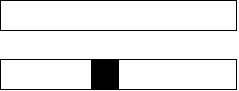
\includegraphics[scale=0.5]{figures/TTPProfiles/initImpl.pdf}} & I am about to & \tabitem Shift H's attention & \tabitem Desire to start \\
                                                & & start speaking & towards T & a conversation \\
																								& & & & \\
						\hline
                                                \rule{0pt}{4ex}
                                                \textbf{DIALOGUE\_INIT} & \multirow{6}{*}{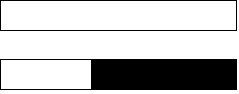
\includegraphics[scale=0.5]{figures/TTPProfiles/init.pdf}} & I start this & \tabitem Shift H's attention & \tabitem Desire to start \\
                                                & & conversation and I & towards T & a conversation \\
                                                & & inform you that x & \tabitem Make H aware & about x \\
                                                & & & of the dialogue & \\
                                                & & & topic (x) & \\
																								& & & & \\
                                                \hline
                                                \rule{0pt}{4ex}
                                                \textbf{FAIL\_IMPL} & \multirow{4}{*}{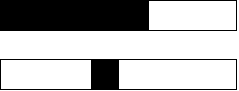
\includegraphics[scale=0.5]{figures/TTPProfiles/implBargeIn.pdf}} & I don't understand & \tabitem Make H stop & \tabitem Fix desynchro- \\
                                                & & what you are & \tabitem Make H repeat & nisation \\
                                                & & talking about & or reformulate & \\
																								& & & & \\
                                                \hline
                                                \rule{0pt}{4ex}
                                                \textbf{FAIL\_RAW} & \multirow{4}{*}{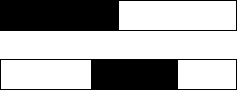
\includegraphics[scale=0.5]{figures/TTPProfiles/shortBargeIn.pdf}} & I don't understand & \tabitem Make H stop & \tabitem Fix desynchro- \\
                                                & & what you are & \tabitem Make H repeat & nisation \\
                                                & & talking about & or reformulate & \\
																								& & & & \\
                                                \hline
                                                \rule{0pt}{4ex}
                                                \textbf{FAIL\_INTERP} & \multirow{8}{*}{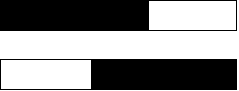
\includegraphics[scale=0.5]{figures/TTPProfiles/longBargeIn.pdf}} & I don't understand & \tabitem Make H stop & \tabitem Fix desynchro- \\
                                                & & what you are & \tabitem Make H repeat & nisation \\
                                                & & talking about & or reformulate & \\
                                                & & because of x & \tabitem Making H aware & \tabitem More efficiency by \\
                                                & & & of what is & providing more \\
                                                & & & preventing T & precision about \\
                                                & & & from understanding & the problem \\
																								& & & & \\
                                                \hline
                                                \rule{0pt}{4ex}
                                                \textbf{INCOHERENCE\_IMPL} & \multirow{5}{*}{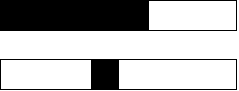
\includegraphics[scale=0.5]{figures/TTPProfiles/implBargeIn.pdf}} & What you just said & \tabitem Make H stop & \tabitem Fix desynchro- \\
                                                & & is problematic & \tabitem Make H reconsider & nisation \\
                                                & & & what he & \\
                                                & & & just said & \\
																								& & & & \\
                                                \hline
                                                \rule{0pt}{4ex}
                                                \textbf{INCOHERENCE\_RAW} & \multirow{5}{*}{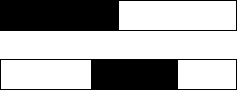
\includegraphics[scale=0.5]{figures/TTPProfiles/shortBargeIn.pdf}} & What you just said & \tabitem Make H stop & \tabitem Fix desynchro- \\
                                                & & is problematic & \tabitem Make H reconsider & nisation \\
                                                & & & what he & \\
                                                & & & just said & \\
																								& & & & \\
                                                \hline
                                                \rule{0pt}{4ex} 
                                                \textbf{INCOHERENCE\_INTERP} & \multirow{8}{*}{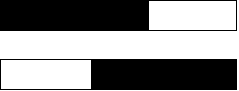
\includegraphics[scale=0.5]{figures/TTPProfiles/longBargeIn.pdf}} & What you just said & \tabitem Make H stop & \tabitem Fix desynchro- \\
                                                & & is problematic & \tabitem Make H reconsider & nisation \\
                                                & & because of x & what he & \tabitem More efficiency by \\
                                                & & & just said & providing more \\
                                                & & & \tabitem Making H aware & precision about \\
                                                & & & of the problem & the problem \\
                                                & & & in his utterance & \\
																								& & & & \\
                                                \hline
                                                \rule{0pt}{4ex}
                                                \textbf{BACKCHANNEL} & \multirow{3}{*}{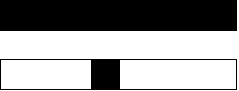
\includegraphics[scale=0.5]{figures/TTPProfiles/backchannel.pdf}} & I understand (and & \tabitem Make H continue & \tabitem More information \\
                                                & & sometimes: I agree) & & from H \\
																								& & & & \\
                                                \hline
                                                \rule{0pt}{4ex}
                                                \textbf{FEEDBACK\_RAW} & \multirow{7}{*}{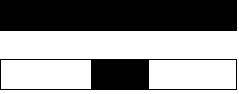
\includegraphics[scale=0.5]{figures/TTPProfiles/shortFb.pdf}} & I understood that & \tabitem Make H continue & \tabitem More information \\
                                                & & you said x & \tabitem Make H correct & from H \\
                                                & & & in case of a & \tabitem Desire to confirm\\
                                                & & & misunderstanding & that H's utterance\\
                                                & & & or not & has been well \\
                                                & & & & understood \\
																								& & & & \\
                                                \hline
					\end{tabular}
				}
				\caption{Taxonomy labels (1/2)}
				\label{tab:taxosynth}
			\end{table}

                        \begin{table}[th]
				\fontsize{8.2}{8.2}
                                \selectfont
				\vspace{2mm}
				\centerline{
					\begin{tabular}{|c|c|c|c|c|}
						\hline
						\textbf{TTP} & \textbf{Locutionary act} & \textbf{Illocutionary act} & \textbf{Perlocutionary act} & \textbf{Motivations} \\
	                                        \hline
																								\rule{0pt}{4ex}
                                                \textbf{FEEDBACK\_INTERP} & \multirow{10}{*}{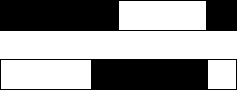
\includegraphics[scale=0.5]{figures/TTPProfiles/longFb.pdf}} & I understood that & \tabitem Make H continue & \tabitem More information \\
                                                & & you said x & \tabitem Make H correct & from H \\
                                                & & that is related  & in case of a & \tabitem Desire to confirm\\
                                                & & to y & misunderstanding & that H's utterance\\
                                                & & & or not & has been well \\
                                                & & & & understood \\
                                                & & & & \tabitem Stronger confirmation \\
                                                & & & & by adding related \\
                                                & & & & information y \\
																								& & & & \\
                                                \hline
																								\rule{0pt}{4ex}
                                                \textbf{REF\_IMPL} & \multirow{6}{*}{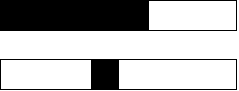
\includegraphics[scale=0.5]{figures/TTPProfiles/implBargeIn.pdf}} & Yes, x & \tabitem Make H stop & \tabitem Selecting an option\\
                                                & & & and understand & \tabitem Less effort as x \\
                                                & & & T is referring to & has already been \\
                                                & & & the last element & uttered by H \\
                                                & & & he uttered (x) & \\
																								& & & & \\
                                                \hline
																								\rule{0pt}{4ex}
                                                \textbf{REF\_RAW} & \multirow{9}{*}{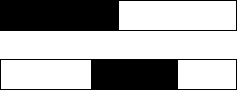
\includegraphics[scale=0.5]{figures/TTPProfiles/shortBargeIn.pdf}} & Yes, x & \tabitem Make H stop & \tabitem Selecting an option\\
                                                & & & and understand & \tabitem Less effort as x \\
                                                & & & T is referring to & has already been \\
                                                & & & the last element & uttered by H \\
                                                & & & he uttered (x) & \tabitem Desire to confirm \\
                                                & & & \tabitem Make H correct & that the last option \\
                                                & & & \tabitem in case of a & has been well \\
                                                & & & misunderstanding & understood \\
																								& & & & \\
                                                \hline
                                                \rule{0pt}{4ex}
                                                \textbf{REF\_INTERP} & \multirow{12}{*}{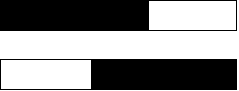
\includegraphics[scale=0.5]{figures/TTPProfiles/longBargeIn.pdf}} & Yes, x that & \tabitem Make H stop & \tabitem Selecting an option\\
                                                & & is related to y & and understand & \tabitem Less effort as x \\
                                                & & & T is referring to & has already been \\
                                                & & & the last element & uttered by H \\
                                                & & & he uttered (x) & \tabitem Desire to confirm \\
                                                & & & \tabitem Make H correct & that the last option \\
                                                & & & \tabitem in case of a & has been well \\
                                                & & & misunderstanding & understood \\
                                                & & & & \tabitem Stronger confirmation \\
                                                & & & & by adding related \\
                                                & & & & information y \\
																								& & & & \\
                                                \hline
                                                \rule{0pt}{4ex}
                                                \textbf{BARGE\_IN\_RESP} & \multirow{10}{*}{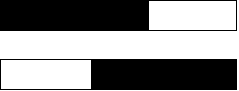
\includegraphics[scale=0.5]{figures/TTPProfiles/longBargeIn.pdf}} & x & \tabitem Make H aware & \tabitem Desire to move \\
                                                & & & of x & the dialogue \\
                                                & & & & forward \\
                                                & & & & \tabitem More efficiency \\
                                                & & & & because enough \\
                                                & & & & information has \\
                                                & & & & been provided before \\
                                                & & & & the end of the \\
                                                & & & & utterance \\
																								& & & & \\
                                                \hline
																								\rule{0pt}{4ex}
                                                \textbf{REKINDLE} & \multirow{6}{*}{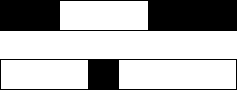
\includegraphics[scale=0.5]{figures/TTPProfiles/rekindle.pdf}} & The information you & \tabitem Make H resume & \tabitem Fix desynchronisation \\
                                                & & gave is not & & \\
                                                & & enough, please & & \\
                                                & & provide more & & \\
                                                & & information & & \\
																								& & & & \\
                                                \hline
                                                \rule{0pt}{4ex}
                                                \textbf{END\_POINT} & \multirow{4}{*}{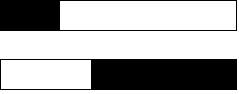
\includegraphics[scale=0.5]{figures/TTPProfiles/endPoint.pdf}} & x & \tabitem Make H aware & \tabitem Desire to move \\
                                                & & & of x & the dialogue \\
                                                & & & & forward \\
																								& & & & \\
                                                \hline
					\end{tabular}
				}
				\caption{Taxonomy labels (2/2)}
				\label{tab:taxosynth2}
			\end{table}
		
     %HK> Réorganiser les sections.
     %HK> Faire un tableau de synthèse de la discussion (avec un niveau d'analyse par colonne par exemple).
     \subsection{Turn-taking phenomena in dialogue systems}
		
          %HK> Rajouter d'autres citations à Raux2008 (Hirschberg...etc...).
          %HK> Le choix du task oriented dialogue est un peu parachuté, profiter du fait que ce soit un chapitre sur la taxonomie pour dire quels phénomènes augmentent le réalisme, quels autres l'efficacité etc... puis introduire notre choix petit à petit.
          INIT\_DIALOGUE is a TTP that is involved in every dialogue system, including traditional ones. There are two ways of initialising the dialogue, the user initiative one (the user starts speaking first like this is the case for Siri for instance) and the system initiative way (the system delivers an initial prompt, when calling an IVR for example). END\_POINT is also necessary for any kind of dialogue, however, the way the dialogue participants exchange turns is not always the same given the situation at hand. Humans are very good at detecting end of utterance clues beforehand, making T able to anticipate the right moment to take the floor hence achieving smooth turn-taking. Traditional dialogue systems, on the other hand, rely on long enough silences as markers of end of turn. A research thread is dedicated to studying methods of reducing these silences by considering different clues (prosodic, lexical and semantic) aiming for smoother turn exchange \cite{Raux2008}. These are good applications of dialogue, and even though they have been under study for many years, there is still room for improvement. However, as we will see later, this is not the focus of this thesis. In the rest of this section, we discuss the remaining TTPs (that can be replicated in incremental dialogue systems only) from an implementation point of view. Our goal is to come up with a list of TTPs that are the most likely to improve task-oriented dialogue. Similarly, REKINDLE is a dialogue management strategy that can be implemented in any traditional dialogue system and as a consequence, it will not be implemented here.

          %HK> Parler du nouveau challenge permettant d'interagir sans casque dans la section dédiée aux challenges relatifs au dialogue incrémental dans le chapitre état de l'art.
          Before leading this discussion, it is important to notice that each TTP has two symmetric versions when it comes to human-machine dialogue: the one where H is the user and T is the machine and the opposite case. In order for both cases to be implemeted, the incremental dialogue system at hand should always be listening to the user, even though it has the floor (hence being able to be interrupted). As a technical side note, current incremental dialogue systems are used with a headphone for that reason: as the system keeps listening all the time, it is a convenient way to prevent it from hearing itself while speaking (considering its own sentence as a user input). In order to make them useful outside of labs, in more realistic situations, it is necessary to build algorithms that suppress the TTS result from the ASR input before feeding it to the latter (which raises a new challenge as it must also be done incrementally). Moreover, in this thesis, the focus is on the vocal modality. Therefore, no TTP based on gestures is considered for implementation.

          %HK> Rajouter une citation pour les incompréhensions de l'ASR.
          Implementing a mechanism that mimics the FAIL TTPs is an interesting idea to explore. Users frequently use off-domain words and expression \cite{Ghigi2014} and they are also ofter misunderstood by the ASR. As a consequence, making the system barge-in when it does not understand the user's partial utterance might have a positive impact on the dialogue efficiency. It might be less tiresome for the user as she wouldn't have to repeat her whole sentence several times. Moreover, this reduces the dialogue duration. FAIL\_RAW is not easy to replicate by a machine and it is most of the time performed with gestures and facial expressions at the same time. FAIL\_INTERP is not easy to implement neither as giving the accurate reason why it did not manage to understand the user's utterance so far is not an obvious task. Implementing FAIL\_RAW, on the other hand, is much more realistic: when the systems has no clue about the user's utterance after a long enough period of time, it simply declares that fact in a straightforward fashion.

          %HK> Référence qui justifie l'existence des cas d'incohérence.
          In some cases, the user is likely to utter a sentence that is not coherent for the system or that is in contradiction with some data accessible by the latter (like when trying to buy a movie ticket when all the seats are already sold). By definition, the INCOHERENCE TTPs can help manage this case in a more efficient way. For the same reasons as FAIL\_RAW, INCOHERENCE\_RAW is not easy to implement. Unlike FAIL TTPs, it is not natural and more difficult to declare an incoherence without explaining the underlying reasons. Therefore, INCOHERENCE\_INTERP is the most interesting TTP to implement.

          %HK> Référence qui justifie que le backchanneling améliore la qualité du dialogue (Meena2013?,Hastie2013).
          %HK> Justifier la correlation entre human-likeness et efficacité (références).
          BACKCHANNEL has already been implemented in a few incremental dialogue systems with the aim of increasing its grounding capacities and its naturalness. This thesis focuses more on the efficiency aspect of incremental dialogue than the human-likeness side of the problem. These are somehow correlated, but as this is not a TTP that directly makes the dialogue more efficienct (by preventing and fixing errors), it will not be implemented. Moreover, as the first step of the approach followed here is to use simulated dialogues, it is hard to evaluate this TTP in such conditions. On the contrary, FEEDBACK\_RAW provides a concrete opportunity to correct errors. When T tries to repeat a part of T's utterance and she succeeds, this gives H a proof that T heard his sentence (even though, this does not necessarily mean that T has well understood the message). If she fails, it is also interesting as H can repeat or refomulate his utterance, hence avoiding a desynchronisation. This is clearly interesting to be implemented in a dialogue system, yet, it can be very challenging. The involved turn-taking mechanism is tricky in the sense that the user should not interpret the system's intervention as a barge-in hence being interrupted. Moreover, the system should be able to recognise whether the user ignored the feedback or tried to correct its content. Therefore, this TTP has been implemented in simulation only. Finally, FEEDBACK\_INTERP requires high NLP capabilities and access to an important knowledge base. Therefore, it has not been implemented here.

          %HK> Revoir toute cette section et discuter des phénomènes symétriques (du côté de l'utilisateur) là où ce n'est pas fait.
          %HK> Rappeler les résultats relatifs à la stratégie incrémentale de Layla.
          In \cite{El-Asri2014a}, REF\_RAW has been implemented from the user's point of view: the system enumerates a list of alternatives and the user barges-in to select one of them. This has been shown to significantly increase the dialogue quality. However, implementing it requires changing the dialogue management strategy whereas, as discussed in Chapter \ref{ch:architecture}, in this study the impact of adding a turn-taking layer on top of pre-existing dialogue management strategies. As a consequence, REF\_IMPL, REF\_RAW and REF\_INTERP are not studied here.

          Finally, BARGE\_IN\_RESP is clearly worth implementing from both sides. From the system's perspective, taking the floor as soon as it has enough information to do so can directly increase dialogue efficiency by reducing dialogue duration but also indirectly by preventing the user from adding new misleading information \cite{Ghigi2014}. From the user's point of view, being able to take the floor before the end of the system's utterance can make the dialogue less tiresome. This is especially true for users that are familiar with the system and as a conseqence, they are able to predict the rest of the systems dialogue acts ahead of time.

          To summarise, four TTP requiring incremental dialogue processing have been selected for rule-based implementation (one of them from both sides: system and user):
          \begin{itemize}
            \item FAIL\_RAW (System side)
            \item INCOHERENCE\_INTEPR (System side)
            \item FEEDBACK\_RAW (System side)
            \item BARGE\_IN\_RESP (System and user side)
          \end{itemize}

          In Chapter \ref{ch:baseline}, the details of the implementation, the rules chosen as well as a comparative study in a simulated environment are provided.
